%!TEX root = ../Project.tex

\subsection{Software overview}
\label{developmentsoftwareoverview}

This section of the report gives an overview of the feature-complete software,
including a walkthrough of the entire selection and allocation process. There
are two parts to the software; an administrative interface (used in the setup
and allocation phases) and a ranking interface (used by the students).

\subsubsection{Setup}

On loading the main administrative page, users are greeted with a form that
allows them to setup the system by uploading their ``assets'' from four
\gls{csv} files (Figure~\ref{walkthrough_admin_main}). Setup is conducted
simply by uploading these four files:

\begin{enumerate}
  \item Sheets (one for each different type of student using the system)
  \item Modules
  \item Groups (one or more per sheet)
  \item Students
\end{enumerate}

\subsubsection{Ranking}

The interface that students use to rank their modules after logging in is
shown in Figure~\ref{walkthrough_student_rank}. The user drags modules from
the left column to the right column using their mouse. For users without
JavaScript enabled in their web browser, a simple \gls{html} form appears
instead of this interface. The screen displayed to students after clicking
``Save choices'' is shown in Figure~\ref{walkthrough_student_confirm}. It
contains one table for each group visible to the student, with the modules
listed in descending order of rank.

Administrators can use the main administrative page
(Figure~\ref{walkthrough_admin_main}) to make a ranking on behalf of a student
-- after clicking ``Make a ranking on behalf of a student'', the application
prompts the administrator for a student username and then displays the
appropriate ranking interface -- identical to the one shown to students.

% A video of the software in use on a touchscreen device is available at...?

\subsubsection{Allocation and export}

Once the allocation period has ended, administrators can return to the main
screen to view all the choices made by students and to perform the allocation
and tweak the results as necessary.
Figure~\ref{walkthrough_admin_view_all_choices} is included to show the scale
of the table containing all choices -- this particular table contains the same
number of choices as were made during the History department's pilot
run\footnote{591 students and 57 modules, totalling approximately 18000
choices as every student did not have to rank every module}.
Figure~\ref{walkthrough_admin_view_all_choices_visible} is a close-up view of
the same choices table, in which every student and the ranks that they gave
their modules are shown.

There is also a table of allocations which is identically structured. The
table is blank to begin with, before allocations have been made.
Figure~\ref{walkthrough_admin_view_all_allocations_bottom} shows the bottom of
the allocations table, including the form that departments use to perform the
allocation. The text input is only relevant to the History department -- the
value entered is used as the ``equity cap'' mentioned in
Section~\ref{sec:algo_constraints}.

% Figures here:

\begin{landscape}
  \begin{figure}
    \begin{minipage}{0.49\linewidth}
      \centering
      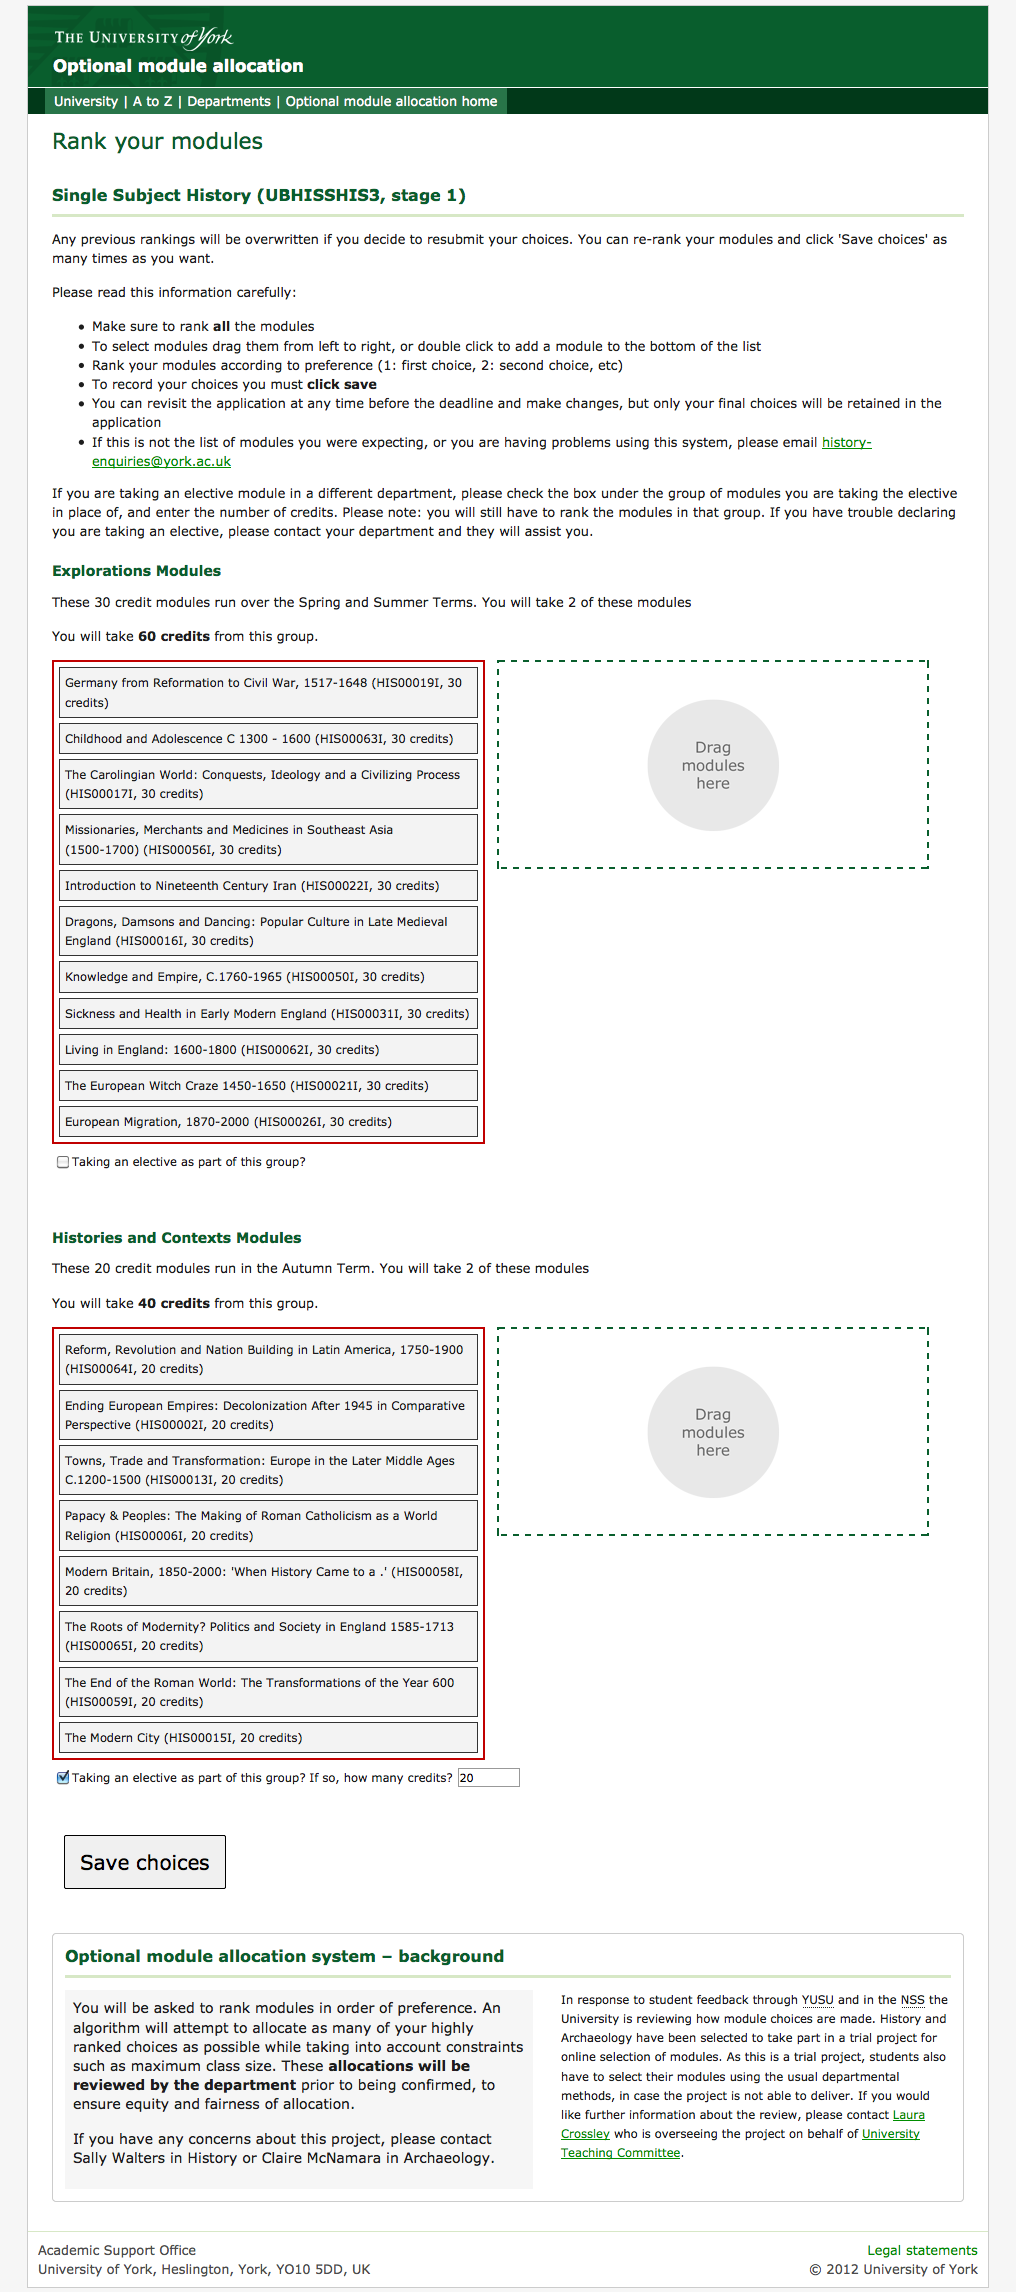
\includegraphics[width=0.6\linewidth]{images/walkthrough/student_rank_modules.png}
      \caption{The student ranking interface}
      \label{walkthrough_student_rank}
    \end{minipage}
    \begin{minipage}{0.48\linewidth}
      \centering
      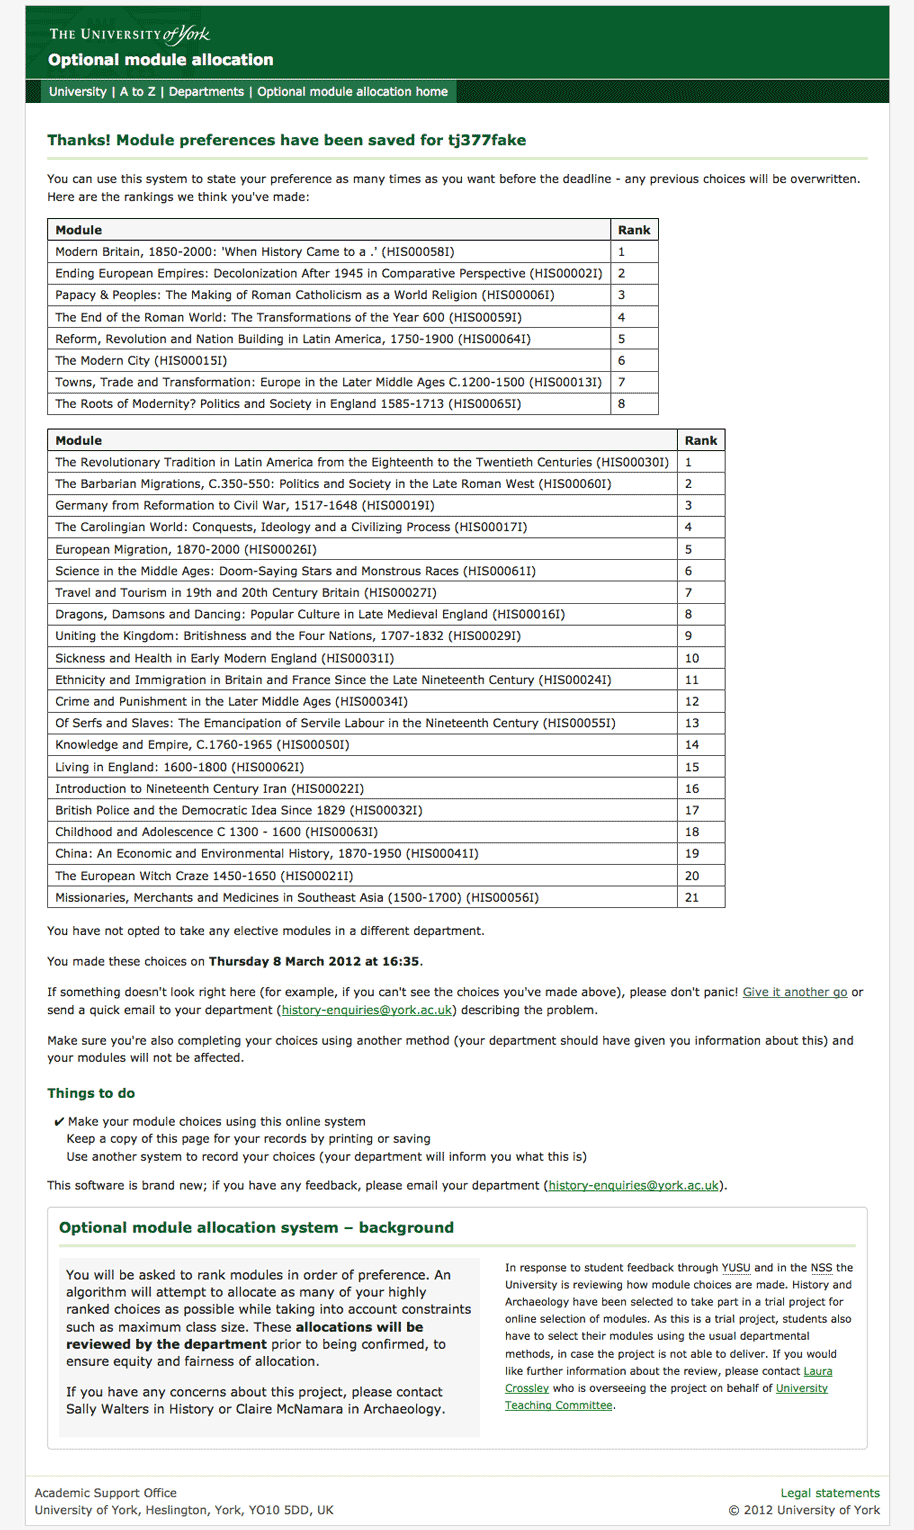
\includegraphics[width=0.8\linewidth]{images/walkthrough/student_confirm_modules.png}
      \caption{The student confirmation interface}
      \label{walkthrough_student_confirm}
    \end{minipage}
  \end{figure}
\end{landscape}

\begin{landscape}
  \begin{figure}
    \begin{minipage}{0.49\linewidth}
      \centering
      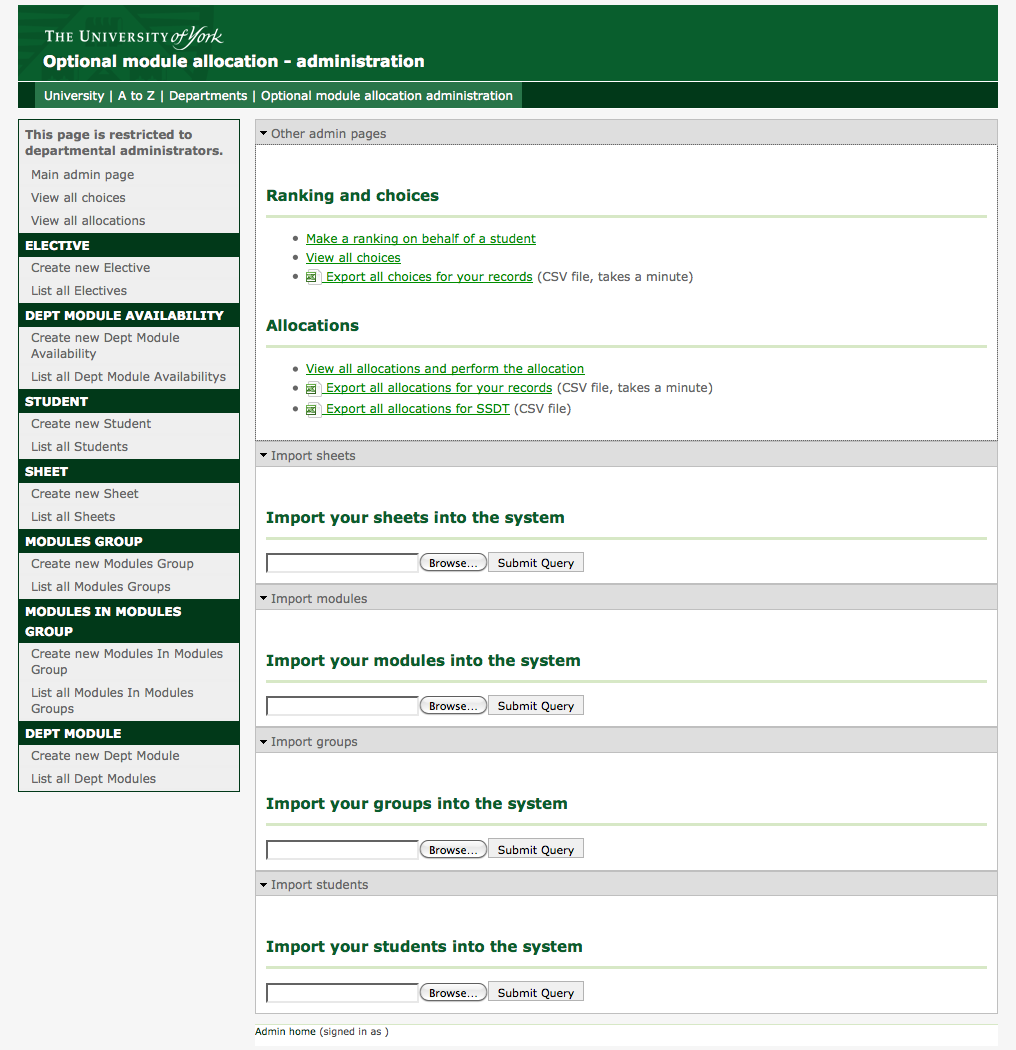
\includegraphics[width=\linewidth]{images/walkthrough/admin_main.png}
      \caption{The main administrative page of the application}
      \label{walkthrough_admin_main}
    \end{minipage}
    \hspace{0.5cm}
    \begin{minipage}{0.48\linewidth}
      \centering
      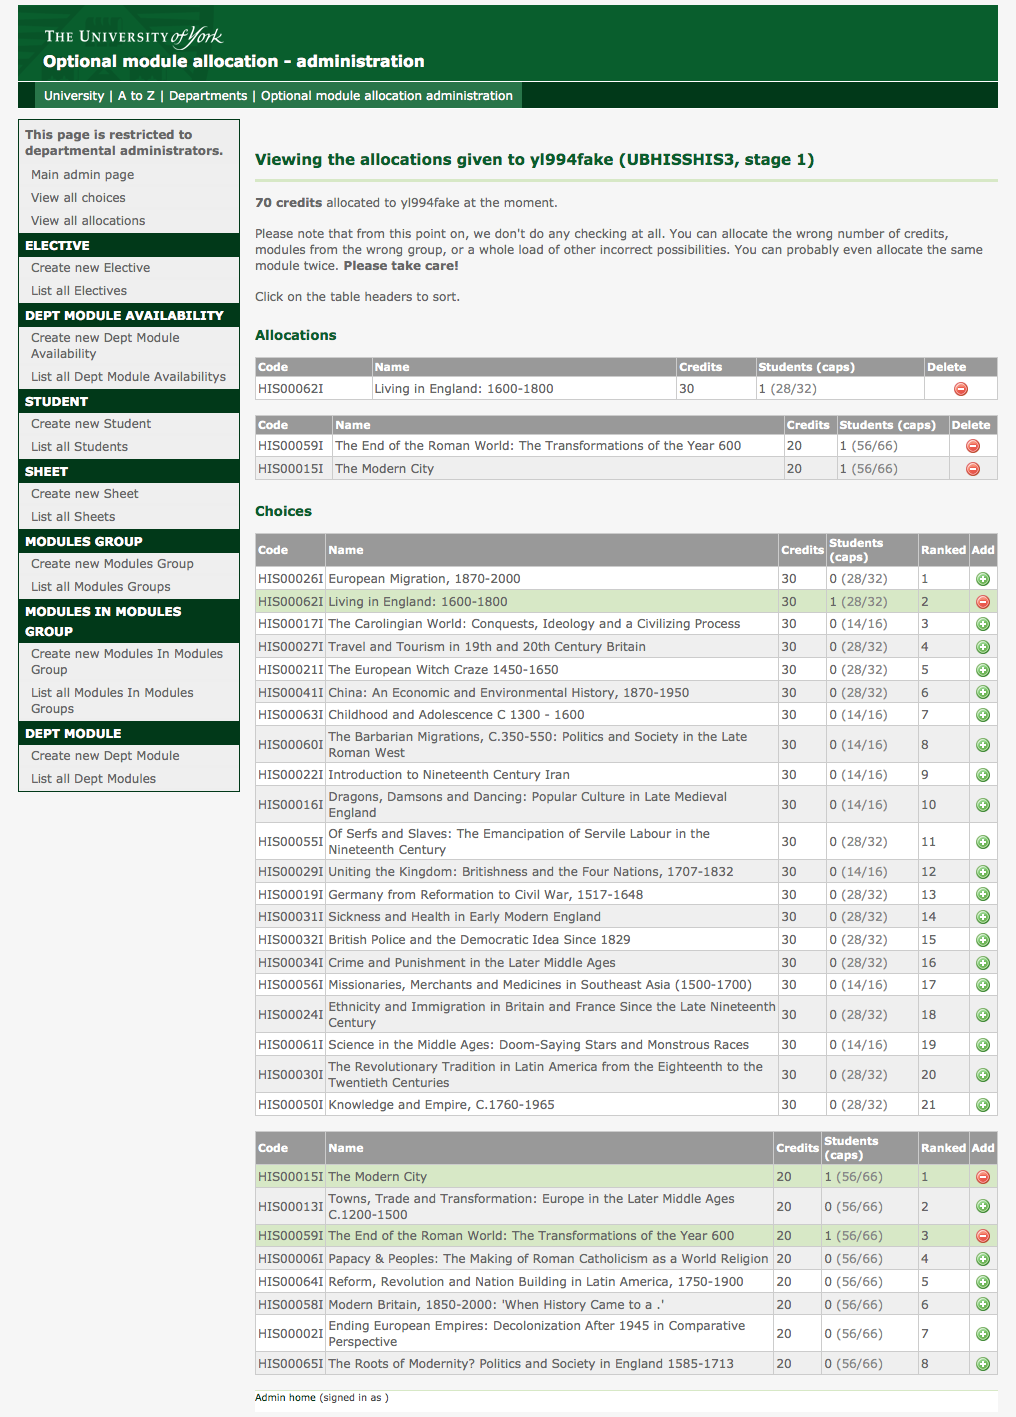
\includegraphics[width=0.9\linewidth]{images/walkthrough/admin_view_student.png}
      \caption{The tweaking view for an individual student}
      \label{walkthrough_admin_view_student}
    \end{minipage}
  \end{figure}
\end{landscape}

\begin{figure}
  \begin{minipage}[]{0.33\linewidth}
    \centering
    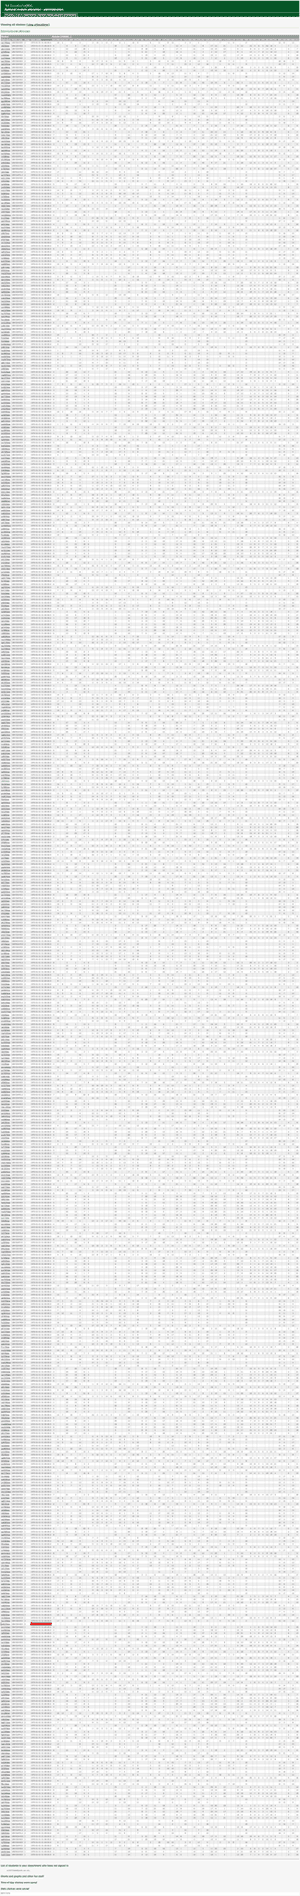
\includegraphics[width=0.6\linewidth]{images/walkthrough/admin_view_all_choices.png}
    \caption{Admin interface showing the number of choices made in the History pilot}
    \label{walkthrough_admin_view_all_choices}
  \end{minipage}
  \hspace{0.1cm}
  \begin{minipage}[]{0.63\linewidth}
    \centering
    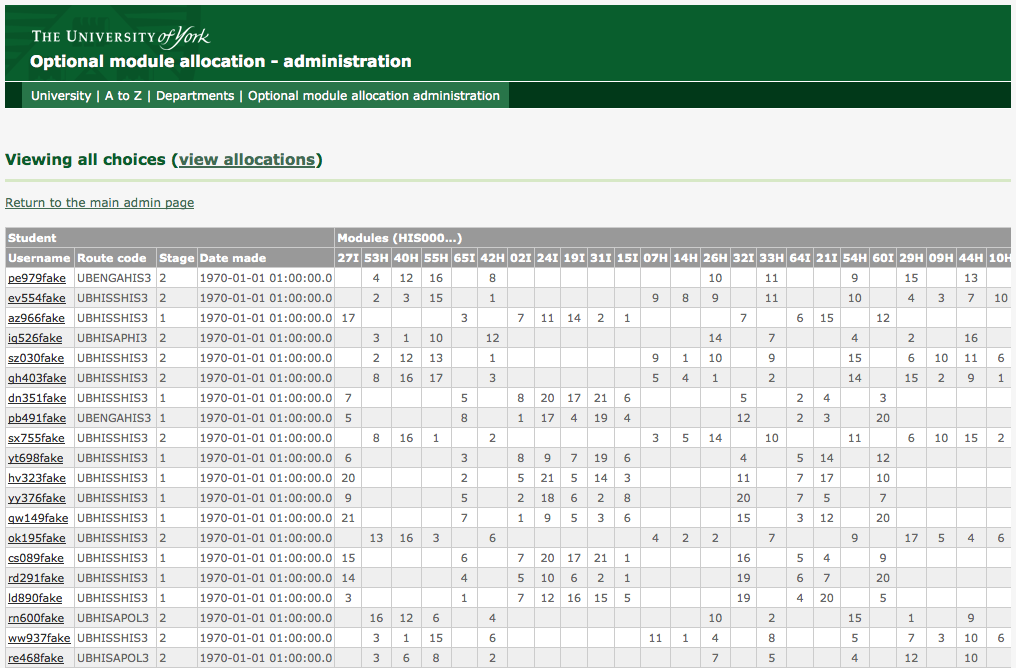
\includegraphics[width=0.9\linewidth]{images/walkthrough/admin_view_all_choices_visible.png}
    \caption{The top of the choices table}
    \label{walkthrough_admin_view_all_choices_visible}
    \bigskip
    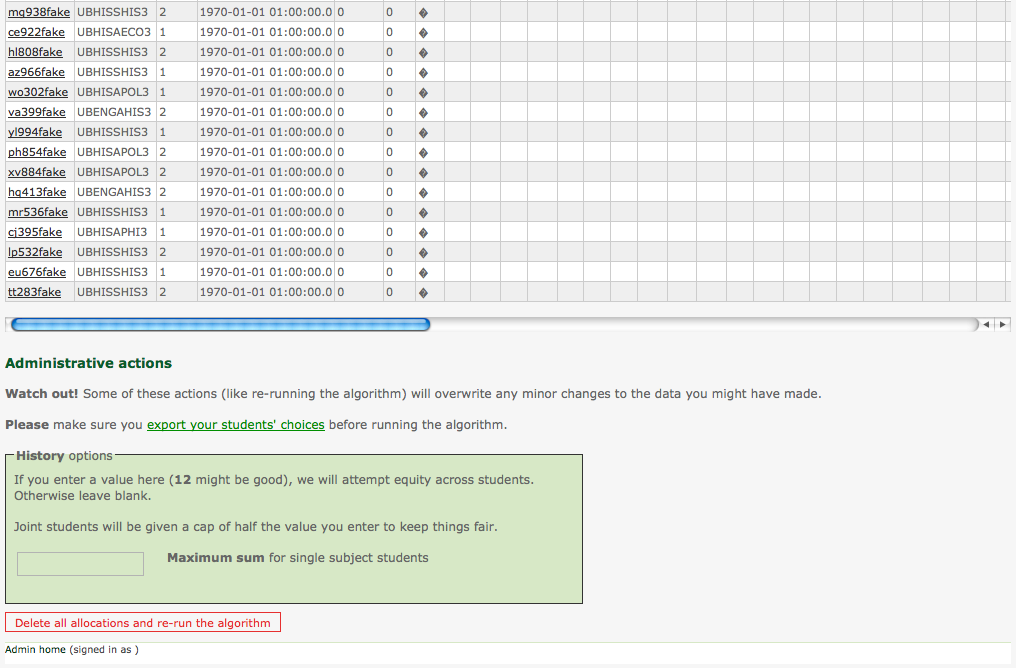
\includegraphics[width=0.9\linewidth]{images/walkthrough/admin_view_all_allocations_bottom.png}
    \caption{The bottom of the allocations table}
    \label{walkthrough_admin_view_all_allocations_bottom}
  \end{minipage}
\end{figure}

Finally, Figure~\ref{walkthrough_admin_view_student} is the tweaking
interface. Once an allocation has been performed, departments can access this
interface by clicking on a student's username. It allows them to delete and
add allocations if they decide they want to make an exception for a particular
module size. Not pictured is the ability to modify module minimum and maximum
sizes and re-run the allocation using these new constraints.

\Gls{csv} files are made available to download using the links on
Figure~\ref{walkthrough_admin_main}. The downloads available are:

\begin{itemize}
  \item A file containing all choices (a table indexed by students and modules)
  \item A file containing all allocations (again, indexed by students and modules)
  \item A list of every allocation made by the system, to be passed to \gls{ssdt}
\end{itemize}
